\documentclass[10pt,journal,compsoc]{IEEEtran}\usepackage[]{graphicx}\usepackage[]{color}
%% maxwidth is the original width if it is less than linewidth
%% otherwise use linewidth (to make sure the graphics do not exceed the margin)
\makeatletter
\def\maxwidth{ %
  \ifdim\Gin@nat@width>\linewidth
    \linewidth
  \else
    \Gin@nat@width
  \fi
}
\makeatother

\definecolor{fgcolor}{rgb}{0, 0, 0}
\newcommand{\hlnum}[1]{\textcolor[rgb]{0,0,0}{#1}}%
\newcommand{\hlstr}[1]{\textcolor[rgb]{0.502,0,0}{#1}}%
\newcommand{\hlcom}[1]{\textcolor[rgb]{0,0,0}{#1}}%
\newcommand{\hlopt}[1]{\textcolor[rgb]{0,0,0}{#1}}%
\newcommand{\hlstd}[1]{\textcolor[rgb]{0,0,0}{#1}}%
\newcommand{\hlkwa}[1]{\textcolor[rgb]{0,0,1}{#1}}%
\newcommand{\hlkwb}[1]{\textcolor[rgb]{0,0,0}{#1}}%
\newcommand{\hlkwc}[1]{\textcolor[rgb]{0,0,1}{#1}}%
\newcommand{\hlkwd}[1]{\textcolor[rgb]{0,0,0}{#1}}%

\usepackage{framed}
\makeatletter
\newenvironment{kframe}{%
 \def\at@end@of@kframe{}%
 \ifinner\ifhmode%
  \def\at@end@of@kframe{\end{minipage}}%
  \begin{minipage}{\columnwidth}%
 \fi\fi%
 \def\FrameCommand##1{\hskip\@totalleftmargin \hskip-\fboxsep
 \colorbox{shadecolor}{##1}\hskip-\fboxsep
     % There is no \\@totalrightmargin, so:
     \hskip-\linewidth \hskip-\@totalleftmargin \hskip\columnwidth}%
 \MakeFramed {\advance\hsize-\width
   \@totalleftmargin\z@ \linewidth\hsize
   \@setminipage}}%
 {\par\unskip\endMakeFramed%
 \at@end@of@kframe}
\makeatother

\definecolor{shadecolor}{rgb}{.97, .97, .97}
\definecolor{messagecolor}{rgb}{0, 0, 0}
\definecolor{warningcolor}{rgb}{1, 0, 1}
\definecolor{errorcolor}{rgb}{1, 0, 0}
\newenvironment{knitrout}{}{} % an empty environment to be redefined in TeX

\usepackage{alltt}
%\documentclass[review,journal]{vgtc}         % review (journal style)
%\documentclass[widereview]{vgtc}             % wide-spaced review
%\documentclass[journal]{vgtc}                % final (journal style)
%\documentclass[preprint,journal]{vgtc}       % preprint (journal style)
%\documentclass[electronic,journal]{vgtc}     % electronic version, journal
%\usepackage{color}
\usepackage{stmaryrd}
\usepackage{stfloats}
%% Uncomment one of the lines above depending on where your paper is
%% in the conference process. ``review'' and ``widereview'' are for review
%% submission, ``preprint'' is for pre-publication, and the final version
%% doesn't use a specific qualifier. Further, ``electronic'' includes
%% hyperreferences for more convenient online viewing.

%% Please use one of the ``review'' options in combination with the
%% assigned online id (see below) ONLY if your paper uses a double blind
%% review process. Some conferences, like IEEE Vis and InfoVis, have NOT
%% in the past.

%% Please note that the use of figures other than the optional teaser is not permitted on the first page
%% of the journal version.  Figures should begin on the second page and be
%% in CMYK or Grey scale format, otherwise, colour shifting may occur
%% during the printing process.  Papers submitted with figures other than the optional teaser on the
%% first page will be refused.

%% These three lines bring in essential packages: ``mathptmx'' for Type 1
%% typefaces, ``graphicx'' for inclusion of EPS figures. and ``times''
%% for proper handling of the times font family.
\usepackage{natbib}
\usepackage{mathptmx}
\usepackage{graphicx}
\usepackage{times}
%% We encourage the use of mathptmx for consistent usage of times font
%% throughout the proceedings. However, if you encounter conflicts
%% with other math-related packages, you may want to disable it.

%% This turns references into clickable hyperlinks.
\usepackage[bookmarks,backref=true,linkcolor=black]{hyperref} %,colorlinks
\hypersetup{
  pdfauthor = {},
  pdftitle = {},
  pdfsubject = {},
  pdfkeywords = {},
  colorlinks=true,
  linkcolor= black,
  citecolor= black,
  pageanchor=true,
  urlcolor = black,
  plainpages = false,
  linktocpage
}

\newcommand{\bitly}[1]{\href{http://bit.ly/#1}{\texttt{#1}}}
\IfFileExists{upquote.sty}{\usepackage{upquote}}{}
\begin{document}

%% If you are submitting a paper to a conference for review with a double
%% blind reviewing process, please replace the value ``0'' below with your
%% OnlineID. Otherwise, you may safely leave it at ``0''.

%% declare the category of your paper, only shown in review mode

%% allow for this line if you want the electronic option to work properly

%% In preprint mode you may define your own headline.
%\preprinttext{To appear in an IEEE VGTC sponsored conference.}

%% Paper title.

\title{Animint: a Grammar for Interactive Animations}

%% This is how authors are specified in the journal style

%% indicate IEEE Member or Student Member in form indicated below
\author{Toby Dylan Hocking,
  Carson Sievert,
  Susan VanderPlas%
\IEEEcompsocitemizethanks{\IEEEcompsocthanksitem
    Toby Dylan Hocking
    is with the McGill University department of Human Genetics,
    Susan VanderPlas and Carson Sievert
    are with Iowa State University department of Statistics.
\protect\\
% note need leading \protect in front of \\ to get a newline within \thanks as
% \\ is fragile and will error, could use \hfil\break instead.
E-mail: toby.hocking@mail.mcgill.ca.}% <-this % stops a space
\thanks{Manuscript received April 19, 2005; revised September 17, 2014.}}

% note the % following the last \IEEEmembership and also \thanks -
% these prevent an unwanted space from occurring between the last author name
% and the end of the author line. i.e., if you had this:
%
% \author{....lastname \thanks{...} \thanks{...} }
%                     ^------------^------------^----Do not want these spaces!
%
% a space would be appended to the last name and could cause every name on that
% line to be shifted left slightly. This is one of those "LaTeX things". For
% instance, "\textbf{A} \textbf{B}" will typeset as "A B" not "AB". To get
% "AB" then you have to do: "\textbf{A}\textbf{B}"
% \thanks is no different in this regard, so shield the last } of each \thanks
% that ends a line with a % and do not let a space in before the next \thanks.
% Spaces after \IEEEmembership other than the last one are OK (and needed) as
% you are supposed to have spaces between the names. For what it is worth,
% this is a minor point as most people would not even notice if the said evil
% space somehow managed to creep in.



% The paper headers
\markboth{Journal of \LaTeX\ Class Files,~Vol.~13, No.~9, September~2014}%
{Shell \MakeLowercase{\textit{et al.}}: Bare Advanced Demo of IEEEtran.cls for Journals}
% The only time the second header will appear is for the odd numbered pages
% after the title page when using the twoside option.
%
% *** Note that you probably will NOT want to include the author's ***
% *** name in the headers of peer review papers.                   ***
% You can use \ifCLASSOPTIONpeerreview for conditional compilation here if
% you desire.



% The publisher's ID mark at the bottom of the page is less important with
% Computer Society journal papers as those publications place the marks
% outside of the main text columns and, therefore, unlike regular IEEE
% journals, the available text space is not reduced by their presence.
% If you want to put a publisher's ID mark on the page you can do it like
% this:
%\IEEEpubid{0000--0000/00\$00.00~\copyright~2014 IEEE}
% or like this to get the Computer Society new two part style.
%\IEEEpubid{\makebox[\columnwidth]{\hfill 0000--0000/00/\$00.00~\copyright~2014 IEEE}%
%\hspace{\columnsep}\makebox[\columnwidth]{Published by the IEEE Computer Society\hfill}}
% Remember, if you use this you must call \IEEEpubidadjcol in the second
% column for its text to clear the IEEEpubid mark (Computer Society journal
% papers don't need this extra clearance.)



% use for special paper notices
%\IEEEspecialpapernotice{(Invited Paper)}



% for Computer Society papers, we must declare the abstract and index terms
% PRIOR to the title within the \IEEEtitleabstractindextext IEEEtran
% command as these need to go into the title area created by \maketitle.
% As a general rule, do not put math, special symbols or citations
% in the abstract or keywords.
\IEEEtitleabstractindextext{%
\begin{abstract}
  Animint is a new domain-specific language (DSL) for linked,
  interactive, animated plots. It builds on top of previous work on
  the grammar of graphics (ggplot2 in R) and interactive visualization
  using web standards (D3 in JavaScript). In other data visualization
  systems, interactive animations are difficult to accomplish, since
  they must be defined in terms of low-level operations and sometimes
  100s of lines of code. In contrast, Animint's high-level DSL can be
  used to produce a wide variety of complex interactive visualizations
  with only 10s of lines of code. It works by adding 2 new aesthetics
  to the grammar of graphics: \texttt{clickSelects}, which allows users to
  select elements of the plot, and \texttt{showSelected}, which displays
  only elements corresponding to the current selection. After using
  the declarative Animint DSL to define an interactive animation in R
  code, it is first compiled and then rendered in a web browser using
  D3. We discuss the design of Animint, then compare to related
  libraries, and show several example visualizations of
  high-dimensional time series data. A free/open-source implementation
  of Animint is available at \url{https://github.com/tdhock/animint}.
\end{abstract}

% Note that keywords are not normally used for peerreview papers.
\begin{IEEEkeywords}
Information visualization, user interfaces, toolkits, 2D
  graphics, interactive, animation
\end{IEEEkeywords}


% make the title area


% To allow for easy dual compilation without having to reenter the
% abstract/keywords data, the \IEEEtitleabstractindextext text will
% not be used in maketitle, but will appear (i.e., to be "transported")
% here as \IEEEdisplaynontitleabstractindextext when compsoc mode
% is not selected <OR> if conference mode is selected - because compsoc
% conference papers position the abstract like regular (non-compsoc)
% papers do!
\IEEEdisplaynontitleabstractindextext
% \IEEEdisplaynontitleabstractindextext has no effect when using
% compsoc under a non-conference mode.


% For peer review papers, you can put extra information on the cover
% page as needed:
% \ifCLASSOPTIONpeerreview
% \begin{center} \bfseries EDICS Category: 3-BBND \end{center}
% \fi
%
% For peerreview papers, this IEEEtran command inserts a page break and
% creates the second title. It will be ignored for other modes.
\IEEEpeerreviewmaketitle

}

%% Keywords that describe your work. Will show as 'Index Terms' in journal
%% please capitalize first letter and insert punctuation after last keyword

%% ACM Computing Classification System (CCS).
%% See <http://www.acm.org/class/1998/> for details.
%% The ``\CCScat'' command takes four arguments.





%% Uncomment below to disable the manuscript note
%\renewcommand{\manuscriptnotetxt}{}

%% Copyright space is enabled by default as required by guidelines.
%% It is disabled by the 'review' option or via the following command:
% \nocopyrightspace

%%%%%%%%%%%%%%%%%%%%%%%%%%%%%%%%%%%%%%%%%%%%%%%%%%%%%%%%%%%%%%%%
%%%%%%%%%%%%%%%%%%%%%% START OF THE PAPER %%%%%%%%%%%%%%%%%%%%%%
%%%%%%%%%%%%%%%%%%%%%%%%%%%%%%%%%%%%%%%%%%%%%%%%%%%%%%%%%%%%%%%%%

%% The ``\maketitle'' command must be the first command after the
%% ``\begin{document}'' command. It prepares and prints the title block.


\maketitle

%% Uncomment below to include a teaser figure.
\begin{figure*}[b!]
  \centering
  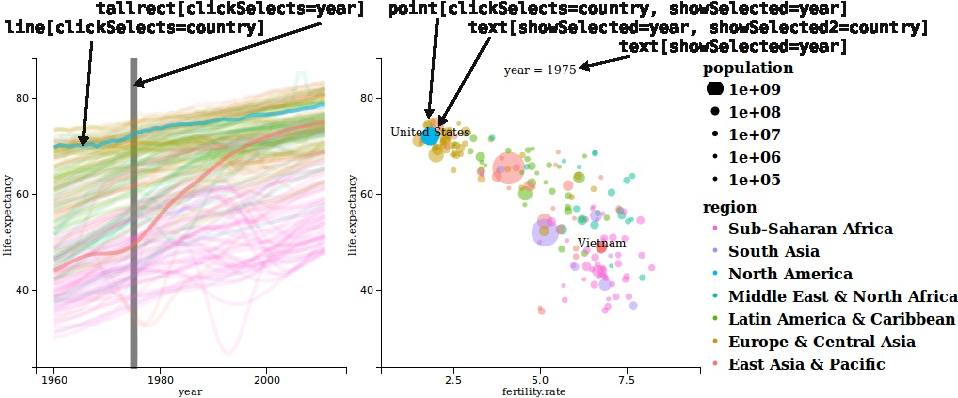
\includegraphics[width=\textwidth]{figure-1}
  \caption{This interactive animation of World Bank data was designed
    with only 20 lines of Animint code (\url{http://bit.ly/worldBank}).
    \textbf{Top text}: Five geometric elements span two linked plots:
    clicking a \texttt{clickSelects} element changes the currently
    selected year or country, and updates the corresponding
    \texttt{showSelected} elements.  \textbf{Left plot}: a multiple
    time series from 1960 to 2012 of the life expectancy of 205
    countries, with bold lines showing the selected countries and a
    vertical grey tallrect showing the selected year.  \textbf{Right
      plot}: a scatterplot of life expectancy versus fertility rate of
    all countries. The two text elements show the current selection:
    year=1975 and country=$\{\textrm{United States},
    \textrm{Vietnam}\}$}
  \label{fig:1}
\end{figure*}

\section{Introduction}

Interactive, animated data visualization is a useful tool for
obtaining an intuitive understanding of patterns in multivariate data
sets. In this paper, we introduce Animint, a system for designing
linked, interactive, animated data visualizations. To demonstrate the
purpose of Animint, we begin with an illustrative example.

The World Bank data set consists of several economic
variables measured for 205 countries from 1960 to 2012
\citep{WorldBank}. Figure~1 shows six variables from this data set:
year, country, life expectancy, fertility rate, region, and
population. In the static PDF version of this figure, the year 1975
and the countries United States and Vietnam are selected, but readers
are encouraged to view and select other countries using a web browser
(\url{http://bit.ly/worldBank}).
%% TODO: Let's update this example and facet the bar chart by region
In the interactive version, the selected value of the year variable is
automatically incremented every few seconds, using animation to
visualize yearly changes in the relationship between life expectancy and
fertility rate. This is just one example in
which interaction and animation help to reveal patterns in a
high-dimensional data set. The Animint system provides a
domain-specific language (DSL) that simplifies the creation of such
interactive and animated data visualizations.

% I wanted to just emphasize the difference between an Animint
% interactive graphic and a static graphic. In static graphics the
% designer chooses both the aes mappings and the subset of data to
% show. However in Animint the designer only chooses the aes mappings
% and then the user is free to choose the selection. Do you have some
% idea how to get that message across?

%% Carson: There are only *two* roles in *creating* visualizations
In general, there are three influential roles involving an Animint
visualization: the developer, who implements the Animint library; the
designer, who uses the Animint library to define a visualization; and
the user, who selects data subsets to view in a web browser. The main
goal of Animint is to provide an expressive language for designers,
while allowing users the freedom to interact with the plot to
selectively view data subsets of interest. The designer specifies data
sets and maps variables to interactive visual elements using the
Animint DSL, then uses the Animint library to compile and save an
interactive animation. The user writes no code, but can view and
interact with an Animint visualization by clicking Scalable Vector
Graphics (SVG) elements in a web browser. The Animint library
developer is responsible for the plot rendering details, which allows
the others to focus on designing and consuming visualizations.

%interested in re-implementing the Animint
%system, we discuss details of its implementation in
%Section~\ref{sec:implementation}.

The Animint DSL is for visualizations which can be both interactive
and animated. For the purposes of this paper, we define
``interactive'' to mean that graphical elements such as data points
may be clicked to update the data that is shown in related plots. This
is closely related to the concept of ``direct manipulation,'' which
was introduced by \citet{shneiderman82} and later applied to
statistical data visualization \citep{Hutchins:1985,
  brushing-scatterplots, cleveland}. Our definition of an ``animated''
visualization is one that can be watched like a video, automatically
updating over time.

%% There is also a very nice discussion about Semantic and
%% Articulatory distance which we could use. Our DSL lowers the
%% semantic distance of the designer, and our renderer lowers the
%% articulatory distance of the user. Mapping the time variable in a
%% data set to the time variable in an animated plot is justified via
%% articulatory directness. Quoting:

%% Semantic distance concerns the relation of the meaning of an
%% expression in the interface language to what the user wants to
%% say. Two important questions about semantic distance are (1) Is it
%% possible to say what one wants to say in this lan- guage? That is,
%% does the language support the user's conception of the task do-
%% main? Does it encode the concepts and distinctions in the domain in
%% the same way that the user thinks about them? (2) Can the things
%% ofintmest be said concisely?  Can the user say what is wanted in a
%% straightforward fashion, or must the user construct a complicated
%% expression to do what appears in the user's thoughts as a
%% conceptually simple piece of work?  ... Where semantic distance has
%% to do with the relationship between user's intentions and meanings
%% of expressions, articulatory distance has to do with the
%% relationship between the meanings of ex- pressions and their
%% physical form. ...  Take the simple, commonplace activity of moving
%% a cursor on the screen. If we do this by moving a mouse, pointing
%% with a finger or a light pen at the screen, or otherwise mimicking
%% the desired motion, then at the level of action execution, these
%% interactions all exhibit articulatory directness. The meaning of
%% the intention is cursor movement and the action is specified by
%% means of a similar movement. One way to achieve articulatory
%% directness at the input side is to provide an interface that
%% permits specification of an action by mimicking it, thus supporting
%% an articulatory similarity between the vocabulary item and its
%% meaning. Any nonarbitrary relationship between the form of an item
%% and its meaning can be a basis for articulatory directness. ...
%% Articulatory directness on the output side is similar. If the user
%% is following the changes in some variable, a moving graphical
%% display can provide articula- tory directness. A table of numbers,
%% although containing the same semantic in- formation, does not
%% provide articulatory directness. Thus, the graphical display and
%% the table of numbers might be equal in semantic directness, but
%% unequal in articulatory directness.

%% Spatial vs temporal indirection:

%% These two types of activation are quite different. The activation
%% of the scrollbar is spatial because it is caused by moving the
%% mouse (and cursor) inside the area of the scrollbar. The activation
%% of the rectangle creation instrument is temporal because it is
%% caused by a former action and remains in effect until the
%% activation of another instrument. (This is traditionally called a
%% mode). Each type of activation has an associated cost: Spatial
%% activation requires the instrument to be visible on the screen,
%% taking up screen real-estate and requiring the user to point at it
%% and potentially dividing the user's attention. Temporal activation
%% requires an explicit action to trigger the activation, making it
%% slower and less direct.  Interface designers often face a design
%% trade-off between temporal and spatial multiplexing of instruments
%% because the activation costs become significant when the user must
%% frequently change instruments. Using extra input devices can reduce
%% these costs. For example, the thumbwheel on Microsoft's
%% Intellimouse is a scrolling instrument that is always active. An
%% extreme example is an audio mixing console, which may contain
%% several hundred potentiometers and switches, each corresponding to
%% a single function. This permits very fast access to all functions,
%% which is crucial for sound engineers working in real-time and
%% cannot afford the cost of activating each function indirectly. A
%% large design space lies between a single mouse and hundreds of
%% potentiometers, posing design challenges to maximally exploit
%% physical devices and reduce activation costs.


%TODO: examples of animated and interactive, World
%Bank and Fig 9 of \citet{d3}.

The type of interactivity that we propose is closely related to the
system described by \citet{cleveland}. In that system, the user's
mouse creates a single rectangular brush which either defines the
selection (transient mode), or defines data points to add to or remove
from the selection (lasting mode or erasing mode). Cleveland also
defines several operations on the selection, such as labeling,
deleting, and enhanced linking. For example, in a scatter plot matrix,
Cleveland uses enhanced linking to highlight which points are selected
in each plot.

In Animint, the central concept of interactivity is a selection
variable, such as year or country in Figure~1. For each selection
variable, one or several values can be selected at a time,
e.g. year=1975 and country=\{United States, Vietnam\}.
Like Cleveland's system, Animint supports enhanced
linking to highlight the selected value(s) of each selection variable. In
contrast to Cleveland's single rectangular brush that selects points in
plots of a single data table, an Animint designer may designate
several selection variables in plots of several linked data tables. To
declare a clickable plot element that changes the selected value of
the year variable, an Animint designer writes
\texttt{clickSelects=year}.
%within a ggplot2 aes specification.

To achieve data-driven animations, Animint defines one other important
operation involving selection variables: showing and hiding subsets of
data in response to user selection. For example, in the scatterplot of Figure~1 we draw a point for
each country, and want to move and change the size of each point as
the selected year changes. To accomplish this, an Animint designer can
simply declare \texttt{showSelected=year} which means to show only the
data with the selected value of year.

Using just the \texttt{clickSelects} and \texttt{showSelected}
keywords, a wide variety of interactive visualizations can be
defined. To make the selection automatically change over time
(animation), an Animint designer may declare one variable as the
\texttt{time} variable. Since it is perceptually advantageous to have
smooth transitions in data-driven animations
\citep{animated-transitions}, an Animint designer may also declare a
\texttt{duration} list of selection variables which should have smooth
transitions.

The Animint DSL is implemented as an extension of ggplot2
\citep{ggplot2-book, ggplot2-paper}, which is a popular R package that
implements the grammar of graphics \citep{wilkinson}. The ggplot2
language was created as a high-level abstraction for non-interactive
visualizations. One of the key strengths of ggplot2 is that it allows
a designer to declare a visualization using multiple layers of
distinct geometric elements, each with a clear aesthetic mapping from
data variables to geometric properties. The Animint DSL extends
ggplot2 by adding \texttt{clickSelects} and \texttt{showSelected}
aesthetics.

\begin{figure*}[b!]
  \centering
  \begin{tabular}{ccc}
  \begin{minipage}{2.5in}
    \centering
    \textbf{D3 (Javascript code)}
    \small
\begin{verbatim}
svg.selectAll("circle")
  .data(one_year)
  .enter().append("circle")
.attr("cx", function(d){
  return x_scale(d.fertility_rate);
}).attr("cy", function(d){
  return y_scale(d.life_expectancy);
}).attr("r", function(d){
  return size_scale(d.population);
}.style("fill", function(d){
  return color_scale(d.region);
})
\end{verbatim}
  \end{minipage}
  &
  \begin{minipage}{2.6in}
    \centering
    \textbf{Vega (JSON file)}
    \small
\begin{verbatim}
{ "marks": [{
  "type":"symbol",
  "from": {"data":"this_year"},
  "properties":{ "enter":{
    "x": {"field": "fertility_rate"},
    "y": {"field": "life_expectancy"},
    "size": {"field": "population"},
    "fill": {"field": "region"}
}}}]}
\end{verbatim}
  \end{minipage}
  &
  \begin{minipage}{2in}
    \centering
    \textbf{Animint (R code)}
    \small
\begin{verbatim}
geom_point(aes(
  x=fertility.rate,
  y=life.expectancy,
  color=region,
  size=population,
\end{verbatim}
    {\color{red}
\begin{verbatim}
  clickSelects=country,
  showSelected=year),
\end{verbatim}
      }
\begin{verbatim}
  data=WorldBank)
\end{verbatim}
    \end{minipage}
  \end{tabular}
  \caption{Comparison of code used to define points on a scatterplot.
    Note that the Animint code is shorter and simpler than the D3 and
    Vega code. Animint and Vega provide nice defaults for plot elements such
    as the axes and labels, but these elements still need to be expressed
    in the D3 code. Also, Animint implements the proposed
    \texttt{clickSelects} and \texttt{showSelected} aesthetics (red),
    but D3 and Vega do not.}
  \label{fig:code}
\end{figure*}

%% Carson: This seems like an opportunity to compare to Vega.
%% Animint is similar in the respect that the renderer takes
%% a JSON object as it's 'input', but it doesn't have the equivalent
%% of Animint's compiler.
The Animint library includes a compiler that converts a list of
ggplots to an interactive web visualization rendered using the
Data-Driven Documents (D3) library for JavaScript \citep{d3}. One of
the main reasons for the success and popularity of D3 is that it
allows visualizations to be specified using the terminology of the
Document Object Model (DOM), which makes learning D3 easy for web
designers. Animint's DSL abandons the DOM standard and sacrifices some
of the flexibility of D3, but it
%reduces the cognitive effort required to create
simplifies creation of visualizations in which users can quickly show/hide
various subsets of data (especially for those familiar with ggplot2).

Finally, another key strength of ggplot2 and D3 for visualization
design are the libraries' declarative syntax, which allows a
visualization designer to specify \emph{what} they want to render
rather than \emph{how} to render it. \citet{declarative} proposed a
declarative syntax for animated transanitions, and studied the
benefits of declarative languages for data visualization. Animint is
another declarative DSL, but defined at a higher level of abstraction
than D3. It enables designers to focus on data visualization, while
the Animint library developers can work on improving the lower-level
rendering details.

The rest of this paper is organized as follows: we discuss related work in
Section~2, and the design of the Animint system in Section~3. Then we
perform a detailed comparison study in Section~4, and
show some example applications of Animint in Section~5. Finally, we
share some user feedback in Section~6 and then discuss future work in
Section~7.

%% \section{Introduction} %for journal use above \firstsection{..} instead

\section{Related Work}

In this section we discuss the differences between Animint and several
related systems, focusing on libraries with free/open-source software
implementations in JavaScript and R.
%% In short, Animint supports many
%% features available in low-level implementations that are not available
%% for higher-level efforts without sacrificing expressiveness.

%% In short, Animint is the first system to propose the clickSelects and
%% showSelected keywords, which simplify the design of a large

\subsection{D3 and other JavaScript libraries}

Animint uses \href{http://d3js.org/}{D3} to render interactive
animations in a web browser \citep{d3}. D3 uses a lower level of
abstraction than Animint, so it is able to express a wider variety of
visualizations. However, Animint can be used to more succinctly
declare certain types of data visualizations. For example,
Figure~\ref{fig:code} shows some Animint and D3 code required to
define the scatterplot in the WorldBank visualization. D3 uses a
data-bind operation followed by several accessor functions, whereas
Animint uses a shorter syntax involving an \texttt{aes} mapping
of data variables to geometric attributes. Importantly, Animint is
able to express interactivity using the simple \texttt{clickSelects}
and \texttt{showSelected} keywords, whereas D3 would require much more
code involving handler functions for mouse click events.

%% Carson: I think this paragraph needs to be a bit more careful/specific
%% with it's claims. For example, ggvis now has linked brushing,
%% Winston Chang presented it at useR 2014 --
%% https://twitter.com/winston_chang/status/484039769265938432
There are many other libraries which can generate web plots with
limited interactivity, but are currently unable to produce interactive
animations. For example, the rCharts R package is a wrapper around
several JavaScript libraries \citep{rcharts}. In contrast to Animint,
rCharts currently does not include heuristics for describing interactions between
multiple plots. Thus, rCharts can easily produce graphics with simple interactive
features (such as tooltips), but it can not produce multi-plot
interactive animations as easily as Animint.

Finally, Dimensional Charting (DC) is another JavaScript library which
can produce interactive visualizations consisting of several linked
plots \citep{dc}. Like Animint, DC builds on top of D3. Unlike
Animint, DC does not use the grammar of graphics, so data
visualization designers are limited to plot types that are pre-defined
by the DC library developers.

\subsection{Animated graphics libraries}

One way to achieve animation in an iterative programming syntax is by
using a for statement to loop over the time variable. This is the main
idea of the \href{http://yihui.name/animation/}{animation} package
\citep{animation}. The main difference between this system
and Animint is that the only interaction possible with
animation is rewinding and fast-forwarding through the
animation frames.

Another way to produce an animated scatterplot of the World Bank data
is by using a Google motion chart, available in R through the
googleVis package \citep{googleVis}. The main limitation of this
system is that it can only produce a few pre-defined plot types, only one
of which can be viewed at any time.

\subsection{Libraries based on the grammar of graphics}

In this section we discuss the differences between Animint and several
other high-level DSLs for data visualization based on the grammar of
graphics \citep{wilkinson}.

\begin{figure*}[p]
  \centering
  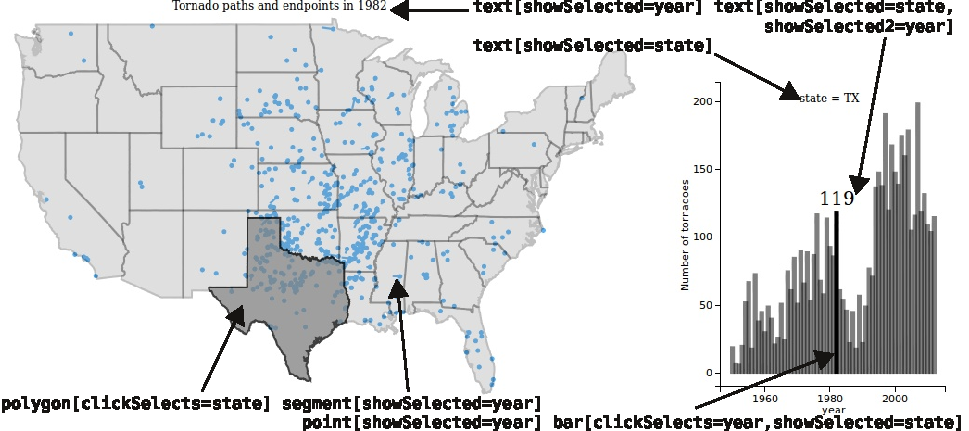
\includegraphics[width=\textwidth]{figure-tornado}
  \caption{Interactive animation of tornadoes recorded from 1950 to
    2012 in the United States (\url{http://bit.ly/1hWvYo0}). \textbf{Left}:
    map of the lower 48 United States with tornado paths in 1982. The
    text shows the selected year, and clicking the map changes the
    selected state, currently Texas. \textbf{Right}: time series of
    tornado counts in Texas. Clicking a bar changes the selected year,
    and the text shows selected state and the number of tornadoes
    recorded there in that year (119 tornadoes in Texas in 1982).}
  \label{fig:tornado}
\end{figure*}

\begin{figure*}[p]
  \centering
  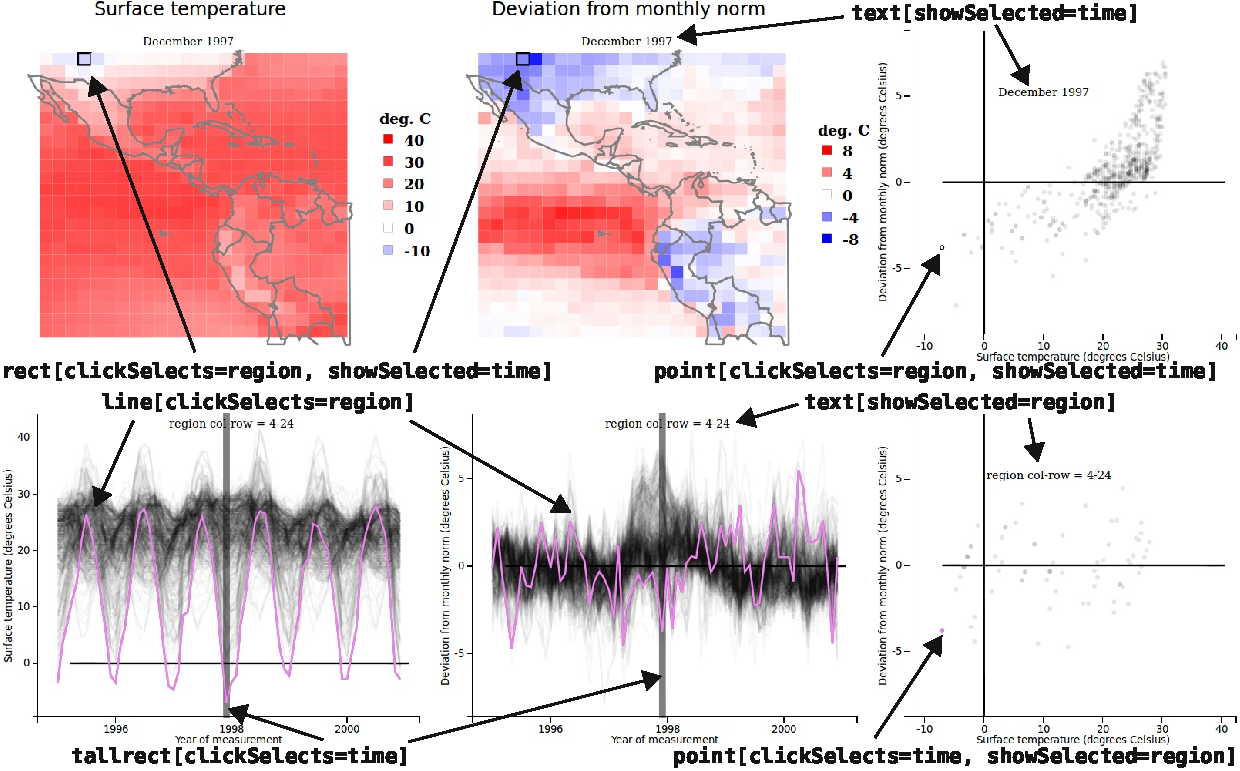
\includegraphics[width=\textwidth]{figure-climate}
  \caption{Visualization containing 6 linked, interactive, animated
    plots of Central American climate data
    (\url{http://bit.ly/QcUrhn}). \textbf{Top}: for the selected time
    (December 1997), maps displaying the spatial distribution of two
    temperature variables, and a scatterplot of these two
    variables. The selected region is displayed with a black outline,
    and can be changed by clicking a rect on the map or a point on the
    scatterplot. \textbf{Bottom}: time series of the two temperature
    variables with the selected region shown in violet, and a
    scatterplot of all times for that region. The selected time can be
    changed by clicking a background tallrect on a time series or a
    point on the scatterplot. The selected region can be changed by
    clicking a line on a time series.}
  \label{fig:climate}
\end{figure*}

Animint extends the declarative DSL of
\href{http://ggplot2.org/}{ggplot2} \citep{ggplot2-book,
  ggplot2-paper}. Strictly speaking, ggplot2 is for non-interactive
and non-animated visualizations. In this paper, we propose the
\texttt{clickSelects} and \texttt{showSelected} aesthetics for
ggplot2, which extend it to accommodate interactive, animated
graphics.

Another R package that uses the grammar of graphics to define
interactive graphics is \href{http://ggvis.rstudio.com/}{ggvis}
\citep{ggvis}. Unlike Animint, ggvis does not directly extend ggplot2,
but provides a new implementation of some of the same ideas about the
grammar of graphics. The main difference is that ggvis relies on
shiny's reactive framework to acheive interactivity
\citep{shiny}. That is, in order to be interactive, ggvis requires a
web server that runs R and shiny. Animint does not require any special
web server software since it uses static files and client-side
JavaScript.

%% Carson: I might be persuaded, but I don't think the argument below will
%% stand the test of time. ggvis is rapidly evolving and already
%% has decent support for 'direct manipulation' and 'linked plots':
%% shiny::runGitHub(repo = "ggvis", username = "rstudio", subdir = "demo/apps/brush-linked")
%% I'll see if I can come up with a ggvis example that is closer to animint's
%% than Susan's current example -- https://srvanderplas.shinyapps.io/ggvis-animint/

%% TDH 20 Nov 2014 Indeed, that ggvis demo/apps/brush-linked is a nice
%% example of (1) direct manipulation, which animint can do and (2)
%% computing something based on the multiple selection, which animint
%% can NOT do, and is discussed in more detail in section 4.2
%% (WorldBank comparison with ggvis/shiny -- the R+shiny web server is
%% slower than client-side JavaScript alone) and future work (Animint
%% can not compute and display 1 thing based on the set of selected
%% values of a multiple selection variable).

The two packages also have different features for interacting with a
data visualization: ggvis uses sliders, checkboxes, and other HTML
form elements, whereas Animint users can directly click the SVG
elements that are used to visualize the data. For example, a ggvis of
the WorldBank data would animate over the years by adding a play/pause
button to a slider widget which controls the selected year. In
contrast, in Animint we used a multiple time series plot where the
year can be selected by directly clicking the data values on the plot
(Figure~1). The Animint plot is thus easier for the user since it has
more articulatory directness \citep{Hutchins:1985}, and less spatial
offset \citep{instrumental-interaction}.

%\paragraph{Vega}
Like Animint, \href{http://trifacta.github.io/vega/}{Vega} is a
declarative DSL that builds on top of D3 \citep{vega}. Vega is unable
to express all plots that can be made using pure D3, but provides a
JSON file format capable of defining many common plots
(Figure~\ref{fig:code}). As discussed in Section~\ref{sec:design},
Animint also internally uses a JSON file to store meta-data about an
interactive animation. The main difference
is that Vega does not support interactions and animation that show and hide
data subsets across multiple linked plots. Finally,
\citet{2014-reactive-vega} proposed some declarative Vega
extensions ``critical for developing interactive data
visualizations.''  Those extensions are defined at a lower level of
abstraction than the \texttt{clickSelects} and \texttt{showSelected}
keywords of Animint.

Implementations of the grammar of graphics system of
\citet{wilkinson} exist as the Visualization Markup Language (ViZml)
and the Graphics Production Language (GPL) in IBM SPSS Statistics
software, but do not support interactive animations.

\subsection{Other systems with interactive selection}

There are many different methods for interactively specifying a set of
selected data points \citep{scented-widgets, heer2008generalized}. A
common interaction involves a rectangular brush that can select
several data points in a single data table \citep{cleveland,
  brushing-scatterplots}, and highlights the selected data points
across several plots. Importantly, Animint supports selecting and
highlighting several different variables (e.g. year and
country), each of which supports either single or multiple
selection. However, the current implementation of Animint does not
support selection using a rectangular brush (users must click each
data point to add/remove it from the set of selected values).

Another system with interactive facilities similar to Animint is
 \citet{tableau}. Like Animint, it has a declarative
interface that can acheive interactive animations.
Tableau is built on top of VizQL, a visual query language
which took influence from Polaris \citep{polaris}.
Visual query languages automatically and dynamically
execute (and, in some cases, cache) database queries
required to render various properties of the user
defined visualization.

Tableau's graphical user interface (GUI) and visual query approach
makes it easy to design several kinds of linked plots, but it does not
easily acheive the same level of flexibility that Animint/ggplot2's
layered grammar of graphics provides. In particular, ggplot2 allows
for each layer of geoms in a plot to have a different data source and
variable mapping, while Tableau requires each mark of a plot to be a
function of a single query result. This results in a substantial
conceptual difference between the selection models of Tableau and
Animint. In Tableau, there is a selection set for each plot, which may
include several different marks. In contrast, Animint keeps track of a
selection set for each selection variable, each of which has
geom-specific effects based on the geom's clickSelects/showSelected
variables.

%% TDH 20 Nov 2014 I feel like the next paragraph is unfair to Tableau
%% in particular and GUIs in general. Yes the GUI is a limitation, but
%% so is the learning curve of the R language and REPL. Can you
%% re-word that to say that GUIs are better for some people and REPLs
%% are better for others? Also if you really want to use REPL I think
%% you should explain what the acronym stands for.

%% Another fundamental limitation to a visual query language is the
%% restriction to database primitives. For instance, suppose
%% we want to visualize the residuals of different models
%% fit to different subsets of the data. This would require us
%% to precompute the residuals using a different language
%% (such as R) and write tables back to the database. This can
%% lead to an inefficient workflow if we aren't interested in
%% keeping certain models/tables. Starting with version 8.1,
%% Tableau does offer R integration, but the types of objects
%% that can be transferred are limited and it removes the REPL
%% environment that R users enjoy.

\section{The Animint system}
\label{sec:design}

In this section we explain the main ideas of how Animint can be used
for interactive animations. We first explain the DSL that a designer
uses to specify an interactive plot, then explain the user interface
for selecting data subsets. Finally, we discuss some implementation
details of the compiler and renderer, which only the Animint
developers need to be concerned about.

\subsection{The Animint grammar for interactive animations}



The main idea of Animint is that a large class of interactive plots
can be specified using just two interactive keywords:
\texttt{clickSelects} and \texttt{showSelected}. For example, after
clicking a \texttt{clickSelects=year} element, the plot
is updated to show only the \texttt{showSelected=year} elements
corresponding to the selected year. These two simple keywords
form the basis of the Animint DSL which makes it easy for designers
to translate ideas into code and then visualizations.

The first step in the design of any data visualization
is usually to make a sketch
of the desired interactive plot on paper or a whiteboard.
In any plot a designer would sketch
the axes, legends, a few geometric elements, and note which variables
will be shown in the linked plots. An Animint designer needs only add
the \texttt{clickSelects} and
\mbox{\texttt{showSelected}} mappings for each geometric element, as shown in
Figures~1, 3, and 4. These notes can be directly translated to
ggplot2 aesthetics in R code, as explained below.

\begin{figure*}[b!]
  \centering
  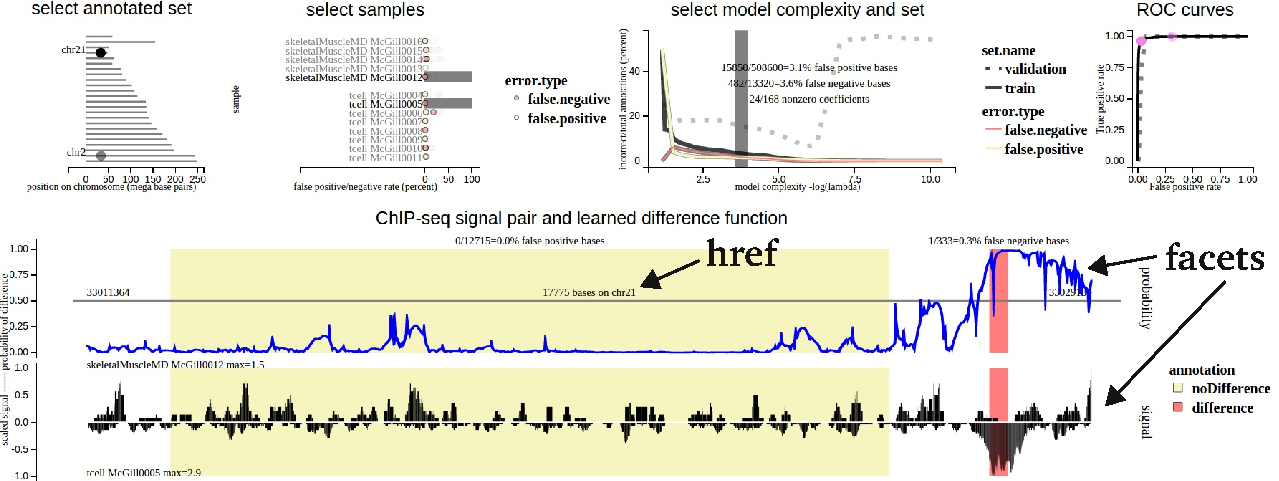
\includegraphics[width=\textwidth]{figure-chip-seq}
  \caption{Visualization with 4 selection variables used to navigate
    through 1,292,464 rows of data in 5 linked interactive plots
    %of a L1-regularized logistic regression model of ChIP-seq data
    (\url{http://bit.ly/1pVZZaS}). The bottom plot shows a
    facets plot with aligned x axes, used to emphasize that the
    blue probability function is defined at the same positions as the
    black signals below. It also contains an href tag (web link), which opens a
    new genome browser web page zoomed to the same region as the
    selected data.}
  \label{fig:ChIPseq}
\end{figure*}

Animint implements the \texttt{clickSelects} and \texttt{showSelected}
interactive keywords as aesthetics in ggplot2. An aesthetic is a
declarative mapping from a data variable to a visual property of a
geometric plot element. Some standard ggplot2 aesthetics are
\begin{description}
\item[x] horizontal position,
\item[y] vertical position,
\item[color] color or fill,
\item[size] point or line thickness.
\end{description}

For example, consider the following R code which defines the points in the
World Bank data scatterplot on the right of Figure~1:

\begin{knitrout}
\definecolor{shadecolor}{rgb}{1, 1, 1}\color{fgcolor}\begin{kframe}
\begin{alltt}
\hlstd{countryPoints} \hlkwb{<-} \hlkwd{geom_point}\hlstd{(}
    \hlkwd{aes}\hlstd{(}\hlkwc{x}\hlstd{=fertility.rate,} \hlkwc{y}\hlstd{=life.expectancy,}
        \hlkwc{color}\hlstd{=region,} \hlkwc{size}\hlstd{=population,}
        \hlkwc{clickSelects}\hlstd{=country,}
        \hlkwc{showSelected}\hlstd{=year),}
    \hlkwc{data}\hlstd{=WorldBank)}
\end{alltt}
\end{kframe}
\end{knitrout}

The code defines a \verb+geom_point+, which means to create a point
for every row in the \texttt{WorldBank} data table. The visual
characteristics of each point are defined by the values of the
corresponding data: the (x,y) position encodes fertility rate and life
expectancy, point color encodes the region, and point size encodes the
population. Note that scales are automatically constructed for the x
and y axes, and legends are automatically constructed for color and
size. The interactivity is also defined as a simple variable mapping:
\texttt{clickSelects=country} means that clicking a point changes the
selected country, and \texttt{showSelected=year} means to only plot
the points for the selected year.

In order to remind the plot user which subset of data are selected, we
will draw a text label with the selected year and country. First, we
create the year labels using

\begin{knitrout}
\definecolor{shadecolor}{rgb}{1, 1, 1}\color{fgcolor}\begin{kframe}
\begin{alltt}
\hlstd{yearText} \hlkwb{<-} \hlkwd{geom_text}\hlstd{(}
  \hlkwd{aes}\hlstd{(}\hlkwc{label}\hlstd{=}\hlkwd{sprintf}\hlstd{(}\hlstr{"year = %d"}\hlstd{, year),}
      \hlkwc{showSelected}\hlstd{=year),}
  \hlkwc{x}\hlstd{=}\hlnum{5}\hlstd{,} \hlkwc{y}\hlstd{=}\hlnum{80}\hlstd{,}
  \hlkwc{data}\hlstd{=years)}
\end{alltt}
\end{kframe}
\end{knitrout}

Note that \texttt{data=years} specifies another data table, with 1 row
for each year. Animint does not require that linked plots originate
from the same data table; the \texttt{clickSelects} and
\texttt{showSelected} aesthetics will work as long as the different
data tables have common variable names (e.g. the \texttt{year}
variable is present in both \texttt{WorldBank} and \texttt{years}).
The \texttt{label} aesthetic is used to define the text from the year
variable, and only the selected year is shown due to the
\texttt{showSelected=year} aesthetic. Finally, note that since the
label \texttt{x} and \texttt{y} positions are constant, they are not
defined as aesthetics.

%% As the pairing of text geom with a corresponding \mbox{showSelected}
%% aesthetic is frequently useful in linked plots, animint also includes
%% a shorthand function to make defining this combination more efficient.

%% <<yearText-make>>=
%% yearText <- make_text(data=years,
%%   x=5, y=80, showSelected="year")
%% @

We can also add another label to show the selected country:

\begin{knitrout}
\definecolor{shadecolor}{rgb}{1, 1, 1}\color{fgcolor}\begin{kframe}
\begin{alltt}
\hlstd{countryText} \hlkwb{<-} \hlkwd{geom_text}\hlstd{(}
    \hlkwd{aes}\hlstd{(}\hlkwc{x}\hlstd{=fertility.rate,} \hlkwc{y}\hlstd{=life.expectancy,}
        \hlkwc{label}\hlstd{=country,}
        \hlkwc{showSelected}\hlstd{=country,}
        \hlkwc{showSelected2}\hlstd{=year),}
    \hlkwc{data}\hlstd{=WorldBank)}
\end{alltt}
\end{kframe}
\end{knitrout}

Note that Animint allows any number of \mbox{showSelected}
aesthetics. In this example, \texttt{showSelected=country} combined
with \texttt{showSelected2=year} means to only show the subset of
labels corresponding to both the selected year and country.  Since
there is only 1 row for each (country, year) combination in the
WorldBank data, this has the effect of drawing the selected country's
label at the location of the selected year.

Having defined these 3 geometric elements, we combine them in a single
ggplot:

\begin{knitrout}
\definecolor{shadecolor}{rgb}{1, 1, 1}\color{fgcolor}\begin{kframe}
\begin{alltt}
\hlstd{scatterPlot} \hlkwb{<-} \hlkwd{ggplot}\hlstd{()}\hlopt{+}
  \hlstd{countryPoints}\hlopt{+}
  \hlstd{yearText}\hlopt{+}
  \hlstd{countryText}
\end{alltt}
\end{kframe}
\end{knitrout}

This completes the definition of the scatterplot. Now, we discuss the
time series on the left of Figure~1. First, the tallrects in the
background are used to select the year:

\begin{knitrout}
\definecolor{shadecolor}{rgb}{1, 1, 1}\color{fgcolor}\begin{kframe}
\begin{alltt}
\hlstd{yearRects} \hlkwb{<-} \hlkwd{geom_tallrect}\hlstd{(}
  \hlkwd{aes}\hlstd{(}\hlkwc{xmin}\hlstd{=year}\hlopt{-}\hlnum{1}\hlopt{/}\hlnum{2}\hlstd{,} \hlkwc{xmax}\hlstd{=year}\hlopt{+}\hlnum{1}\hlopt{/}\hlnum{2}\hlstd{,}
      \hlkwc{clickSelects}\hlstd{=year),}
  \hlkwc{data}\hlstd{=years,} \hlkwc{alpha}\hlstd{=}\hlnum{1}\hlopt{/}\hlnum{2}\hlstd{)}
\end{alltt}
\end{kframe}
\end{knitrout}

%Animint is designed for
%interactivity via direct manipulation of the plot elements.
%To facilitate this goal,
The tallrect is an Animint extension useful for selecting the variable
which is plotted on the x axis, such as \texttt{year} in this
example. The tallrect plots a rectangle for every row of the
\texttt{years} data table. The rectangle spans the entire y region,
and the \texttt{xmin} and \texttt{xmax} aesthetics define the left and
right limits. Since the designer specified \texttt{clickSelects=year},
users can click on a tallrect to select a year.
%% Finally,
%% \texttt{alpha=1/2} specifies that the selected tallrect should have an
%% opacity of 50\%. Since color is black by default, this results in a
%% selected semi-transparent tallrect which appears grey. Since
%% non-selected \texttt{clickSelects} plot elements have 1/2 less opacity
%% by default, this results in non-selected rectangles which are
%% completely transparent, blending in with the white background.


%% Animint also provides a shorthand syntax for tallrects, as they are a
%% common geom/aesthetic pairing in linked plots.

%% <<yearRects-make>>=
%% yearRects <- make_tallrect(WorldBank, "year")
%% @

%% This approach allows us to utilize both plots to display meaningful
%% information: we can overlay the tallrects in the first plot with time
%% series data while still using the tallrects to modify the second
%% plot. Similar linked graphs could be produced with D3, but the grammar
%% of graphics approach allows for fewer lines of code and simpler
%% debugging.

To create the time series plot, we combine the tallrects above with
lines. To declare that clicking a line should change the selected
country, we use the \texttt{clickSelects=country} aesthetic:

\begin{knitrout}
\definecolor{shadecolor}{rgb}{1, 1, 1}\color{fgcolor}\begin{kframe}
\begin{alltt}
\hlstd{timeSeries} \hlkwb{<-} \hlkwd{ggplot}\hlstd{()}\hlopt{+}
  \hlstd{yearRects}\hlopt{+}
  \hlkwd{geom_line}\hlstd{(}
    \hlkwd{aes}\hlstd{(}\hlkwc{x}\hlstd{=year,} \hlkwc{y}\hlstd{=life.expectancy,}
        \hlkwc{group}\hlstd{=country,} \hlkwc{color}\hlstd{=region,}
        \hlkwc{clickSelects}\hlstd{=country),}
    \hlkwc{data}\hlstd{=WorldBank,} \hlkwc{size}\hlstd{=}\hlnum{3}\hlstd{,} \hlkwc{alpha}\hlstd{=}\hlnum{3}\hlopt{/}\hlnum{5}\hlstd{)}
\end{alltt}
\end{kframe}
\end{knitrout}

Note that both the \texttt{timeSeries} and \texttt{scatterPlot}
objects are valid ggplots. However, plotting them using the standard
ggplot2 library will show a non-interactive plot will all
geometric elements, including data for all years and countries. To
plot them with Animint, we define a list of ggplots and options, then
call the \texttt{animint2dir} compiler:

\begin{knitrout}
\definecolor{shadecolor}{rgb}{1, 1, 1}\color{fgcolor}\begin{kframe}
\begin{alltt}
\hlstd{viz} \hlkwb{<-}
  \hlkwd{list}\hlstd{(}\hlkwc{scatterPlot}\hlstd{=scatterPlot,}
       \hlkwc{timeSeries}\hlstd{=timeSeries,}
       \hlkwc{time}\hlstd{=}\hlkwd{list}\hlstd{(}\hlkwc{variable}\hlstd{=}\hlstr{"year"}\hlstd{,} \hlkwc{ms}\hlstd{=}\hlnum{3000}\hlstd{),}
       \hlkwc{duration}\hlstd{=}\hlkwd{list}\hlstd{(}\hlkwc{year}\hlstd{=}\hlnum{1000}\hlstd{))}
\hlkwd{animint2dir}\hlstd{(viz,} \hlkwc{out.dir}\hlstd{=}\hlstr{"WorldBank"}\hlstd{)}
\end{alltt}
\end{kframe}
\end{knitrout}

The \texttt{time} option specifies that in absence of user
interaction, we want the plots to animate over time, progressing at a
rate of one year every 3 seconds. We also use the \texttt{duration}
option to specify a smooth transition over 1 second for the year
variable. The \texttt{animint2dir} compiler saves some data files and a
web page in the \texttt{WorldBank} directory, then it opens the
interactive plot in a web browser.

\subsection{User interaction}

\citet{instrumental-interaction} discussed the advantages of direct
manipulation in graphical user interfaces, and our Animint system
follows principle 2 ``Physical actions on objects vs. complex syntax''
such as dialog boxes. In particular, the user can update the selection
by clicking on the data objects themselves. This contrasts other
systems which use menus and widgets, and thus suffer from less
articulatory directness \citep{Hutchins:1985}.

For single selection variables such as year, clicking sets the value
of the corresponding selection variable. For multiple selection
variables such as country, clicking adds or removes values from the
set of selected values.


\subsection{Implementation details}
\label{sec:implementation}

As shown in Figure~\ref{fig:design}, the Animint system is implemented
in 2 parts: the compiler and the renderer.

\begin{figure}[b!]
  \centering
  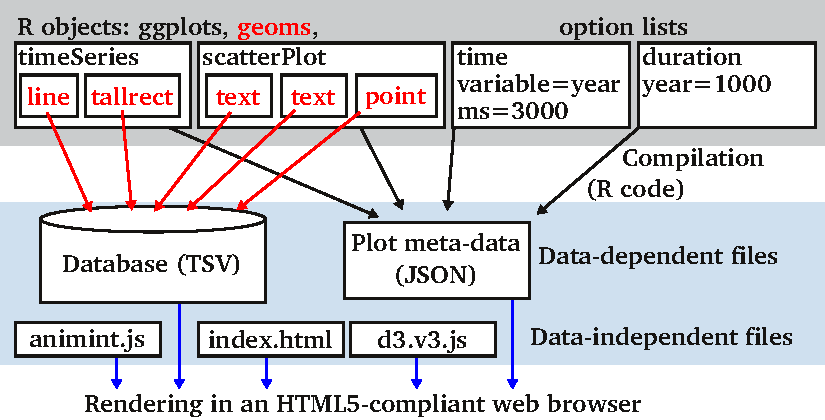
\includegraphics[width=\columnwidth]{figure-design}
  \caption{Schematic explanation of compilation and rendering the
    World Bank visualization shown in Figure~1. \textbf{Top}: the
    interactive animation is a list of 4 R objects: 2 ggplots and 2
    option lists. \textbf{Center}: Animint R code compiles data in
    ggplot geoms to a database of TSV files
    (\textcolor{red}{$\rightarrowtriangle$}). It also compiles plot
    meta-data including ggplot aesthetics, animation time
    options, and transition duration options to a JSON meta-data file
    ($\rightarrowtriangle$). \textbf{Bottom}: those data-dependent
    compiled files are combined with data-independent JavaScript and
    HTML files which render the interactive animation in a web browser
    (\textcolor{blue}{$\rightarrowtriangle$}).}
  \label{fig:design}
\end{figure}

The compiler is implemented in about 1500 lines of R code that
converts a list of ggplots and options to a tab-separated values
(TSV) file database and a JSON plot meta-data file. The compiler scans
the aesthetics in all of the ggplots to determine how many selection
variables are present, and which plots to update after a selection
variable is clicked. It uses ggplot2 to automatically calculate
the axes scales, legends, and labels. It outputs this information to
the JSON plot meta-data file. It also uses ggplot2 to convert data
variables (e.g. life expectancy and region) to visual properties
(e.g. y position and color). The data are separated into several TSV
files, so for large data sets the web browser only needs to download
the subset of data required to render the current selection
\citep{2013-immens}. Finally, the rendering engine
(\texttt{index.html}, \texttt{d3.v3.js}, and \texttt{animint.js}
files) is copied to the plot directory. Since the compiled plot is
just a directory of files, the designer can easily upload interactive
plots to any web server.% for sharing with users.

The \texttt{animint.js} renderer is implemented in about 1500 lines of
JavaScript/D3 code that renders the TSV and JSON plot data files as
SVG in a web browser.
%% The main idea for implementing interactivity is
%% that clicking a \texttt{clickSelects=year} geom calls the
%% \verb|update_selector| function, which stores the newly selected value
%% of year, then calls \verb|update_geom| to redraw every geom with
%% \texttt{clickSelects=year} or \texttt{showSelected=year}.
Importantly, animation is achieved by using the JavaScript
\texttt{setInterval} function, which updates the \texttt{time}
selection variable every few seconds.

\section{Results and comparison study on World Bank data}
\label{sec:compare}

To show the advantages that the Animint grammar brings for creating
interactive and animated data visualizations, we implemented the World
Bank visualization of Figure~1 using two other R packages and Tableau
(Table~\ref{tab:packages}). The main result of our comparison is that
Animint requires significantly fewer lines of code, and produces
interactive plots with more articulatory directness
\citep{Hutchins:1985}. Note that is it possible to implement the World
Bank visualization in pure D3 (Figure~\ref{fig:code}), but would
require significantly more code.

\subsection{R package animation}
\label{sec:compare-animation}

We designed a version of the WorldBank visualization with limited
interactivity, using 38 lines of R code and the \texttt{animation}
package (\url{http://bit.ly/1hnUnkE}). The main idea behind this
approach is to use an imperative programming style with for loops to
create a static PNG image for each year of the data, and then show
these images in sequence. The main drawback to this approach is that
the resulting plot is only interactive with respect to the year
variable. In other words, the designer must select some countries to
emphasize, and the user can not change that selection. Another
drawback is that R package \texttt{animation} does not support smooth
transitions between animation frames. In contrast, using only 20 lines
of the Animint DSL, the Animint package achieves smooth transitions
and interaction with respect to both year and country variables.

\begin{table}[t!]
%% Table captions on top in journal version
  \caption{Implementation complexity and features
    of the World Bank data visualization
    %of Figure~1
    using several libraries that can create interactive animations.
    For each library
    we show the number of lines of code (LOC), the on-screen objects
    that can be clicked,  the
    number of interaction variables, and URL of the interactive version.
%  Note that different countries can not be interactively selected using
% the visualization created with R package animation.
  }
 \label{tab:packages}
 \scriptsize
 \begin{center}
  \begin{tabular}{cccccc}
    library &
    LOC &
    click on &
    %language &
    %years &
    interaction vars &
    http://bit.ly/
    \\
    \hline
    animint &
    20 &
    plotted data &
    %R &
    %2013- &
    several &
      \bitly{worldBank}
    \\
    animation &
    38 &
    play/pause &
    %R  &
    %2007- &
    1 = time &
    \bitly{1hnUnkE}
    \\
    %% D3 &
    %% TODO &
    %% JavaScript &
    %% %2011- &
    %% several &
    %% %declarative &
    %% \\
    ggvis/shiny &
    84 &
    widgets &
    %R  &
    %2012- &
    several &
    \bitly{1diUYsg}
    \\
    Tableau &
      &
    widgets/plot &
    several &
    \bitly{worldBank-tableau}
    \\
  \end{tabular}
 \end{center}
\end{table}

\subsection{Client-server systems like ggvis/shiny}

We designed another version of the World Bank data visualization in 84
lines of R code (\url{http://bit.ly/1diUYsg}), using the ggvis
graphics library combined with the recommended shiny web server
package \citep{shiny, ggvis}. Showing and hiding data subsets was
accomplished by clicking on a slider for year and a menu for country,
not by clicking on the plot elements. In contrast, we designed
Figure~1 using only 20 lines of R code with the Animint package. 
Implementation is significantly simpler using Animint
because Animint's DSL is designed specifically for this type of
interactive animation.
%Although creating such visualizations in ggvis+shiny is
%possible, it requires significantly more work for limited
%interactivity.

Another difference is the amount of work required to deploy or share a
visualization. A compiled Animint visualization consists of static
TSV, JSON, HTML, and JavaScript files which can be easily served with
any web server. In contrast, ggvis+shiny requires a web server with R
and special software installed, significantly complicating
deployment to the web.

There are also inherent speed tradeoffs to using a client-server
plotting system like ggvis+shiny rather than an entirely web
client/JavaScript-based system like Animint. There is one main
difference between these two types of systems that affects
responsiveness of a web-based interactive plotting system:
client-server communication overhead. All the \mbox{Animint}
JavaScript plot rendering code is executed in the web browser, whereas
ggvis executes some computations on the server. This means that after
a mouse click, ggvis can not update a plot immediately, but instead
must wait for the server to respond with the plot data.

We quantified speed differences between the two systems by timing web
page loading using DevTools in the Chromium web browser Version
33.0.1750.152, on Ubuntu 12.04 (256984). We also used \texttt{getTime()}
in JavaScript to record timings for interactive plot updates (on a
desktop computer with a 2.8GHz Intel Core i7 CPU). Using ggvis with a
local web server and the World Bank data resulted in a web page that
loaded quickly (about 1.4s), but updated the plot with a noticeable
lag after each mouse click (500--1000ms). Note that since we used a
local web server, these times represent the overhead of the web server
system, and would be larger with a remote web server.

\begin{table*}[b!]
  \centering
  % latex table generated in R 3.0.2 by xtable 1.7-3 package
% Fri Mar 21 10:48:45 2014
\begin{tabular}{rrrrrrrrrrr}
  \hline
 & lines of R code & seconds & MB & rows & onscreen & variables & interactive & plots & animated? & Fig \\ 
  \hline
worldPop & 17 & 0.2 & 0.1 & 924 & 624 &  4 &  2 &  2 & yes &  \\ 
  WorldBank & 20 & 2.5 & 2.3 & 34132 & 11611 &  6 &  2 &  2 & yes &  1 \\ 
  evolution & 25 & 24.7 & 12.5 & 240600 & 2703 &  5 &  2 &  2 & yes &  \\ 
  change & 36 & 3.4 & 2.7 & 36238 & 25607 & 12 &  2 &  3 & no &  \\ 
  tornado & 39 & 1.7 & 6.2 & 103691 & 16642 & 11 &  2 &  2 & no &  2 \\ 
  prior & 54 & 0.8 & 0.2 & 1960 & 142 & 12 &  3 &  4 & no &  \\ 
  breakpoints & 66 & 0.6 & 0.3 & 4242 & 667 & 13 &  2 &  3 & no &  \\ 
  compare & 66 & 12.2 & 7.8 & 133958 & 2140 & 20 &  2 &  5 & no &  \\ 
  climate & 87 & 14.6 & 21.5 & 253856 & 88980 & 15 &  2 &  6 & yes &  3 \\ 
   \hline
\end{tabular}

  \vskip 0.2cm
  \caption{Characteristics of eleven interactive visualizations designed with
    Animint. From left to right, we show the data set name, the
    lines of R code including data processing but not including comments
    (80 characters max per line),
    the amount of time it takes to compile the visualization (seconds),
    the total size of the uncompressed TSV files in megabytes (MB),
    the total number of data points (rows),
    the median number of data points shown at once (onscreen),
    the number of data columns visualized (variables),
    the number of clickSelects/showSelected variables (interactive),
    the number of linked panels (plots),
    if the plot is animated,
    and the corresponding Figure number in this paper (Fig).
  }
\label{tab:examples}
\end{table*}

When we used Animint to make the World Bank data visualization, the
compilation from R objects to 2.1MB of uncompressed TSV data files
took 2.3s. Using a local web server, the Animint JavaScript rendered
the plot very quickly (100--200ms). We also observed very fast plot
updates after mouse clicks in Animint: 20--30ms response times for
selecting the year, and 60--70ms response times for selecting the
country.
%Furthermore, in web server systems the client may not cache
%previously viewed subsets, which results in calculations inefficiently
%being performed several times rather than simply saved for quick
%viewing later.

The conclusion of our speed comparison is that the overhead of waiting
for a web server to perform computations results in significant
slowdowns for interactive animations. It is clear that for quick
response times, it is preferable to use an entirely JavaScript-based
system like Animint.

In contrast, a web server system like ggvis+shiny would be more
appropriate for
%  interactive animations that have many more subsets of
% the data than can ever be transferred over the network. In that case,
% the web server will initially send only the first data subset, and
% then send only the subsets of data that the client requests. However,
% since the data sets we examined were not too large
% (Table~\ref{tab:examples}), client-side rendering using Animint
% resulted in quick, responsive interactive animations.
% Another application for which a web server system like ggvis+shiny
% would be preferable is for
performing arbitrary calculations in R/C code on the server, in
response to user inputs, and then sending the result across the
network for plotting in the user's web browser. This power is not
always necessary for interactive animations, since the only operation
needed is showing precomputed data subsets. However, the web server
system would certainly be preferable when there are many more data
subsets than could ever be precomputed. In that case, the web server
would only compute the subsets that the user interactively specifies.

\subsection{Tableau}

We implemented a version of the WorldBank data visualization using
Tableau's GUI (\url{http://bit.ly/worldBank-tableau}).
%% TDH 20 Nov 2014: When I click on a country on the scatterplot it
%% does not select that country's time series --- is that an inherent
%% limitation of Tableau that we should discuss?
It was impossible to implement all features of the multiple time
series plot of the data visualization, since it includes multiple
layers with different data sources and variable mappings (a line for
each country and a tallrect for each year). Since each mark in a
Tableau plot is limited to a single data source, it was impossible to
control the clickable multiple time series and the clickable tallrects
in different ways based on the two different selection variables. In
conclusion, although Tableau is useful for many simple interactive
data visualizations, it is inherently limited in ways that Animint is not.

\section{Example applications}

In this section we discuss the range of examples that we have designed
with Animint. Table~\ref{tab:examples} shows several characteristics
of eleven interactive visualizations that we have designed using
Animint.

We quantified the implementation difficulty of the Animint examples
using lines of R code, including data processing but not including
comments (80 characters max per line). We counted the number of plots
and variables shown to quantify the amount of information conveyed by
the visualization. Using only 17 lines of code, we designed a simple
visualization that shows 2 linked plots of 4 variables in the worldPop
data set. In contrast, the most complex visualization required 229
lines of code, and it shows 44 variables across 5 linked plots
(Figure~\ref{fig:ChIPseq}). All of the visualizations that we designed
involved at least 2 interaction variables (e.g. year and country in
Figure~1) and 2 plots. Indeed, Animint is most appropriate for
interactive visualizations of multi-variate data that are not easy to
view all at once in one plot.

Table~\ref{tab:examples} also shows Animint system requirements for
plots of various sizes. We timed the compilation step in R code
(``seconds'' column), and measured the size in megabytes of the
compiled TSV file database (``MB'' column), and found that both
increase with the data set size (``rows'' column).
%Although we do not present timings for the rendering step,
We also noticed that the time required for the interactive updates and
rendering increases with the amount of data displayed at once
(``onscreen'' column). In particular, the climate data visualization
has noticeably slow animations, since it displays about 88980
geometric elements at once (\url{http://bit.ly/QcUrhn}). We observed
this slowdown across all browsers, which suggested that there is an
inherent bottleneck when rendering large interactive plots in web
browsers using JavaScript and SVG. Another Animint with a similar
amount of total rows is based on the evolution data
(\url{http://bit.ly/O0VTS4}), but since it shows less data onscreen
(about 2703 elements), it exhibits faster responses to interactivity
and animation.

\subsection{Animated examples}

Animation is very useful for data sets which have a time variable,
as in the World Bank data of Figure~1.

Figure~\ref{fig:tornado} shows an interactive animation of tornadoes
observed in the United States between 1950 and 2012. At any moment in
time, the user can simultaneously view the spatial distribution of
tornadoes in the selected year over all states, and see the trend over
all years for the selected state. Clicking a state on the map updates the
time series bars to show the tornado counts from that state. Clicking
a bar on the time series updates the selected year.

Figure~\ref{fig:climate} shows an interactive animation of climate
time series data observed in Central America. Two maps display the
spatial distribution of two temperature variables, which are shown
over time in corresponding the time series plots below. Scatterplots
also show the relationships between the two temperature variables, for
the selected time and region. Clicking any of the plots updates all 6
of them. The \texttt{clickSelects} and \texttt{showSelected} aesthetics make it easy to
design this set of 6 linked plots in only 87 lines of code.
%% Animint's
%% DSL allows for this level of flexibility while using minimal lines of
%% code to define the plots and the relationship between them.

\subsection{Non-animated examples}

Animint is still useful for creating interactive but
non-animated plots when there is not a time variable in the data. 
In fact, seven of the eleven examples in
Table~\ref{tab:examples} are not animated. For example, linked plots
are useful to illustrate complex concepts such as a change point
detection model in the breakpoints data
(\url{http://bit.ly/1gGYFIV}). The user can explore different model
parameters and data sets since these are encoded as Animint
interaction variables.

Another non-animated example is Figure~\ref{fig:ChIPseq}, which was
used to explain a complex machine learning model for predicting
differences between samples. The interactive visualization allows the
user to explore how the predictions change as a function of the model
complexity parameter, in several train and test samples. It also uses
facets, a feature from ggplot2 that allows multi-panel plots with
aligned axes. Finally, it includes hyperlinks which open related web
pages in new windows.

Overall, we have found that Animint is useful for exploring
relationships in many different kinds of multivariate data. By using
\texttt{clickSelects} and \texttt{showSelected}, it is easy to design
interactive plots that reveal patterns in complex data.

\section{User feedback and observations}

By working with researchers in several fields of research,
we have created a wide variety of
interactive visualizations using Animint.
Typically, the researchers have a complex data set that
they wish to visualize,
but they do not have the expertise or time to create
an interactive data visualization.
The Animint DSL made it easy to collaborate with the various domain experts,
who were able to provide us with annotated sketches of the desired plots,
which we then translated to Animint R code.
In this section we share comments and
constructive criticism that we have obtained from our users.

\subsection{Designer perspective}

R users have found that Animint is easy to learn. One statistics
Ph.D. student writes, ``animint is a fantastic framework for creating
interactive graphics for someone familiar with R and ggplot2's grammar
of graphics implementation. The API is very intuitive and allows one
to quickly bring their static graphics to life in a way that
facilitates exploratory data analysis.''

TODO: expand to address reviewer comments.

\subsection{User perspective}

For the \texttt{prior} data visualization
(\url{http://bit.ly/1peIT7t}), the Animint user is a machine learning
researcher who developed an algorithm and applied it to 4 benchmark
data sets. He wanted to explore how his algorithm performed, in
comparison to a baseline learning algorithm. He appreciated the
intuition about his algorithm's performance that he learned from the
interactive plots: ``Interactive plotting allows us to explore all
relationships of our high-dimensional dataset and gives us an
intuitive understanding of the performance of our proposed
algorithm. An intuitive understanding of the results is important
since it shows under which conditions our proposed method works well
and provides avenues for further research.''

Another user from a machine learning background found the interactive
plots useful for presenting his work: ``the `regularization path' is a
difficult concept to demonstrate in my research. The [Animint
\url{http://bit.ly/1gVb8To}] helped greatly by rendering an
interactive plot of regularization path, likelihood, and graph at the
same time and illustrating their connections. It also reveals an
interesting phenomenon that maximizing the testing likelihood actually
gives many false positives.''

In another application, the Animint user was a genomics researcher:
``viewing and exploring my complex intestinal microbiome dataset in
[Animint] allowed me to grasp the patterns and relationships between
samples at an almost intuitive level. The interactive aspect of it was
very helpful for browsing through the dataset.''

Finally, users also appreciated the simple web interface, and the
detail that is possible to show in interactive plots, but impossible
to show in publications: ``...  the web interface is simple and easy
to use.  It also enables us to publish more detailed interactive
results on our website to accompany the results presented in
publications.''

\section{Limitations and future work}

There are several limitations to the Animint system, which suggest
avenues for future work. Some limitations are specific to the current
implementation as research software, and some limitations are inherent
in the clickSelects/showSelected keywords.

\subsection{Limitations of current implementation}

Animint implements several linked plots, one of the hallmarks of
interactive visual analysis \citep{iva}. However, one limitation to
the current implementation is that a selection is defined as a set of
distinct elements (e.g. year=\{1991, 1992\}) rather than a logical
expression (e.g. year $>1990$). Also, Animint does not yet
implement a rectangular brush for specifying values of
multiple selection variables.
Importantly, these are drawbacks of the
current implementation, not the Animint DSL.

A number of limitations derive from the fact that some plot elements
are computed once during the compilation step and remain static on a
rendered plot. For example, users are unable to change variable
mappings since these are specified by the designer at compile
time. Also, when different data subsets have very different ranges of
values, it may be preferable to recompute scales when
\texttt{clickSelects} selection(s) change. A workaround is shown in
Figure~\ref{fig:ChIPseq}, which omits the x axis on the bottom plot,
since in fact the x values are all normalized to [0,1]. A future
implementation of Animint would benefit from changes to the compiler
and renderer that allow scales to be updated after each click.

Some Animint limitations can be resolved by Animint designers who are
familiar with the shiny web server R package \citep{shiny}.  Animint
provides ``shiny bindings'' which enables a designer to embed an
Animint plot within a shiny app without writing any HTML or
JavaScript, which allows a user to re-compile an Animint from a web
browser. For example, we implemented a shiny app in which users can
redefine variable mappings (\url{http://bit.ly/animint-shiny}).

As discussed in Section~\ref{sec:design} and illustrated in
Figure~\ref{fig:design}, the compiler is written in R, and the
renderer is written in JavaScript.
%% This means that Animint developers must be proficient in both R and
%% JavaScript. This represents a significant barrier for source code
%% contributions from developers who are proficient with one language
%% but not the other.
Animint designers define interactive animations using only R code, and
no knowledge of JavaScript is necessary. This is convenient for useRs
from a statistical background, but presents a barrier for web
developers who are more familiar with JavaScript than R. For these web
developers, it would be advantageous in the future to implement a
compiler and renderer in pure JavaScript, by possibly building
\texttt{clickSelects} and \texttt{showSelected} extensions into Vega
\citep{vega}.

The current Animint implementation is limited to two specific types of
interactivity: highlighting the selected \texttt{clickSelects}
element, and showing/hiding \texttt{showSelected} elements. In the
future, we could implement several other types of interactivity
without changing the Animint DSL. Examples include zooming,
panning, and plot resizing. However, some
kinds of interactivity would require extensions to the Animint
grammar. For example, a \texttt{hoverSelects} aesthetic
could be used to change the selection when hovering over a data point.

\subsection{Limitations of clickSelects/showSelected keywords}

TODO. discuss that grand tours are awkward in animint since each
animation frame must be pre-computed, and there are many more possible
It's not that they can't be computed beforehand. But if you have a
large amount of projections that you want to view, that could be a
bottleneck \citep{tourr}. The grand tour picks random projections, so
I'm pretty sure the number of projections is infinite in the
mathematical sense But there are also guided tours that pick
"interesting" projections.

TODO: discuss two main failure modes: 1. you really want to compute
something on the fly (like a random projection) and 2. with multiple
selection variables, there are too many items in the power set so they
can't all be computed in advance.

TODO: discuss conditioning on quantitative variables? any concrete
example plots where this would be useful? 

TODO: distinction between the clickSelects/showSelected keywords and
the animint system which pre-computes everything? Could there be a
clickSelects/showSelected system which does NOT pre-compute
everything?

Since Animint does not perform any computations other than showing and
hiding data subsets, there is a limitation to what can be
displayed with multiple selection variables.
The limitation is that it is not feasible to precompute
something to display for each of the combinatorial number of
possible selections
of a multiple selection variable.
For instance, in the
WorldBank visualization of Figure~1, it would not be feasible to
display a single smoothing line computed from all the selected
countries. This is because \texttt{showSelected=country} means to show
one thing for each selected country (not one thing computed based on
the set of selected countries). Supporting this kind of interaction
would require substantial modifications to the Animint system,
including adding the ability to perform computations on
multiple selection variable sets.

TODO: revise paragraph. Animint's performance can be measured using
speed, memory, and disk space requirements in the compilation and
rendering steps. Although we showed in Section~\ref{sec:compare} that
Animint provides smoother interactivity than client-server systems,
future versions of Animint could be made even more efficient and
responsive. For example, of the plots in Table~\ref{tab:examples}, the
longest compilation step took 56.3 seconds, which may be reduced by
optimizing the R code compiler.

This highlights one of the main motivations for using a declarative
DSL like Animint: none of the designer's R code needs to be changed to
implement improvements like this. Instead, the Animint developers just
need to work on a better compiler and rendering engine. Indeed,
\citet{declarative} noted that this is one of the main benefits of
declarative language design: ``By decoupling specification from
implementation, developers can implement language optimizations
without interfering with the work of designers.''

While several
optimizations remain to be implemented, the current Animint library
already provides an efficient syntax for the design of interactive,
animated data visualizations.

in the future, I'd be interesting in trying to "solve" (1) for some
class of problems where you want some elements to have smooth
transitions when new data arrives.

\section*{Acknowledgements}

The authors wish to thank Animint users MC Du Plessis, Song Liu,
Nikoleta Juretic, and Eric Audemard
who have contributed constructive criticism and helped its development.

% TDH 13 March 2014 This was in the template.tex file.
%\bibliographystyle{abbrv}

\bibliographystyle{abbrvnat}

%%use following if all content of bibtex file should be shown
%\nocite{*}
\bibliography{refs}
\end{document}
